\documentclass{article}
\usepackage[utf8]{inputenc}
\usepackage{tikz}
\usepackage[T1]{fontenc}
\usepackage{float}
\usetikzlibrary{shapes.geometric, arrows}
\pagenumbering{gobble}

%Node dimensions
\newcommand\nodewidth{.25\linewidth}
\newcommand\nodeheight{.125\linewidth}
\newcommand\nodespacing{1.4}

\tikzstyle{startstop} = [ellipse, minimum width=\nodewidth, minimum height=\nodeheight, text centered, draw=black, fill=white]
\tikzstyle{io} = [trapezium, trapezium left angle=70, trapezium right angle=110, minimum width=\nodewidth, minimum height=\nodeheight, text centered, draw=black, fill=white]
\tikzstyle{process} = [rectangle, minimum width=\nodewidth, minimum height=\nodeheight, text centered, draw=black, fill=white]
\tikzstyle{decision} = [diamond, minimum size=\nodeheight, text centered, draw=black, fill=white]
\tikzstyle{connector} = [circle, minimum size=\nodeheight, text centered, draw=black, fill=white]

\tikzstyle{arrow} = [thick,->,>-stealth]

\begin{document}

\begin{center}

    \begin{figure}[H]
        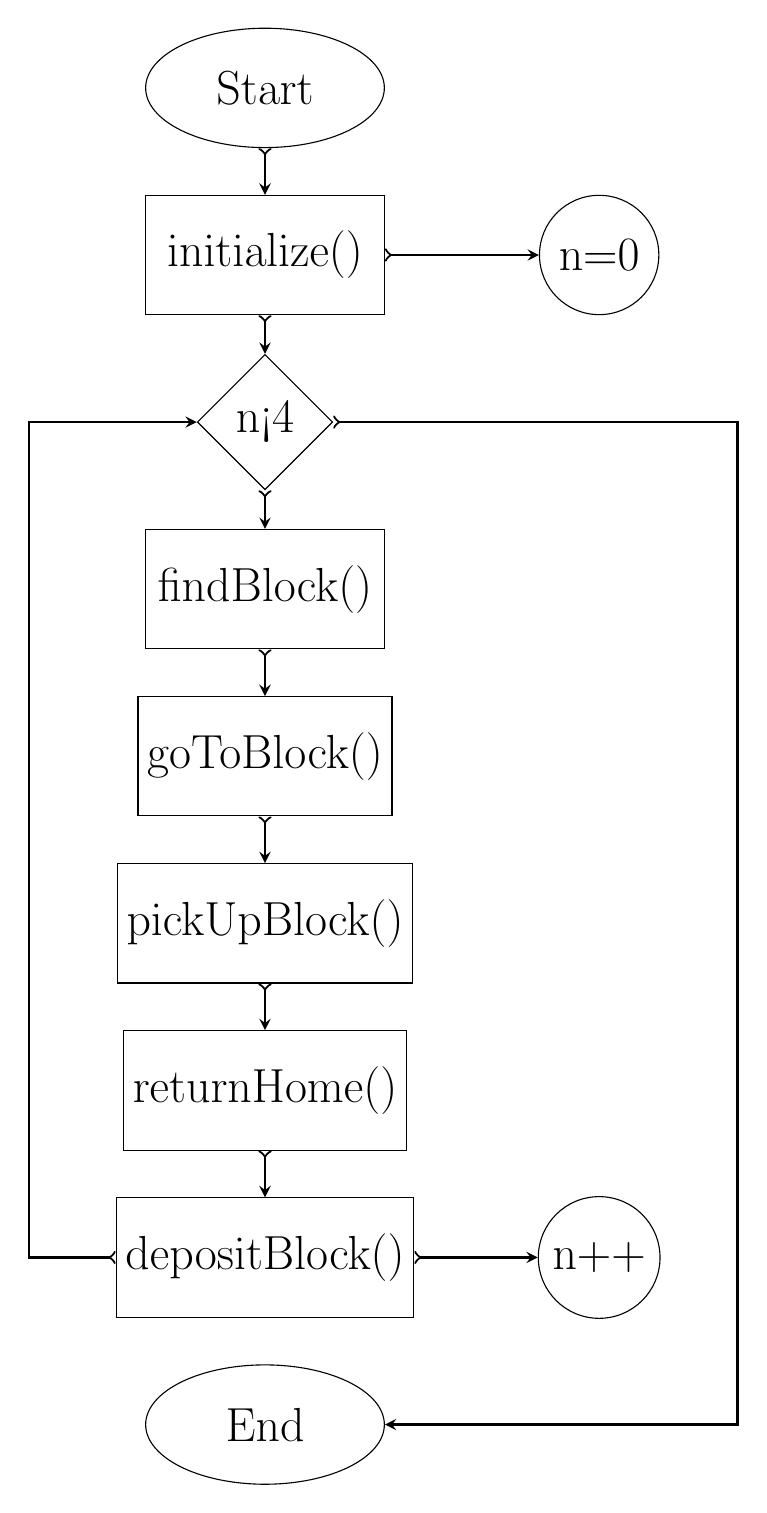
\begin{tikzpicture}[node distance=\nodespacing*\nodeheight]

            \node (start) [startstop]{\LARGE Start};
            \node (initialize) [process, below of=start]{\LARGE initialize()};
            \node (n) [connector, below of=start, xshift=2*\nodespacing*\nodeheight]{\LARGE n=0};
            \node (n<4) [decision, below of=initialize]{\LARGE n<4};
            \node (find) [process, below of=n<4]{\LARGE findBlock()};
            \node (go) [process, below of=find]{\LARGE goToBlock()};
            \node (pickup) [process, below of=go]{\LARGE pickUpBlock()};
            \node (return) [process, below of=pickup]{\LARGE returnHome()};
            \node (deposit) [process, below of=return]{\LARGE depositBlock()};
            \node (n++) [connector, below of=return, xshift=2*\nodespacing*\nodeheight]{\LARGE n++};
            \node (end) [startstop, below of=deposit]{\LARGE End};


            \draw [arrow] (start) -- (initialize);
            \draw [arrow] (initialize) -- (n);
            \draw [arrow] (initialize) -- (n<4);
            \draw [arrow] (n<4) --([shift={(6cm,0mm)}]n<4.center) -- ([shift={(6cm,0mm)}]end.center) -- (end.east);
            \draw [arrow] (deposit) --([shift={(-3cm,0mm)}]deposit.center) -- ([shift={(-3cm,0mm)}]n<4.center) -- (n<4);
            \draw [arrow] (n<4) -- (find);
            \draw [arrow] (find) -- (go);
            \draw [arrow] (go) -- (pickup);
            \draw [arrow] (pickup) -- (return);
            \draw [arrow] (return) -- (deposit);
            \draw [arrow] (deposit) -- (n++);

        \end{tikzpicture}
    \end{figure}
    
\end{center}

\end{document}

